\documentclass[tikz,border=12pt]{standalone}
\usepackage[T1]{fontenc}

\definecolor{ink}{HTML}{253341}
\definecolor{espresso}{HTML}{A56A43}
\definecolor{milk}{HTML}{5689B4}
\definecolor{cold}{HTML}{38A99B}

\begin{document}
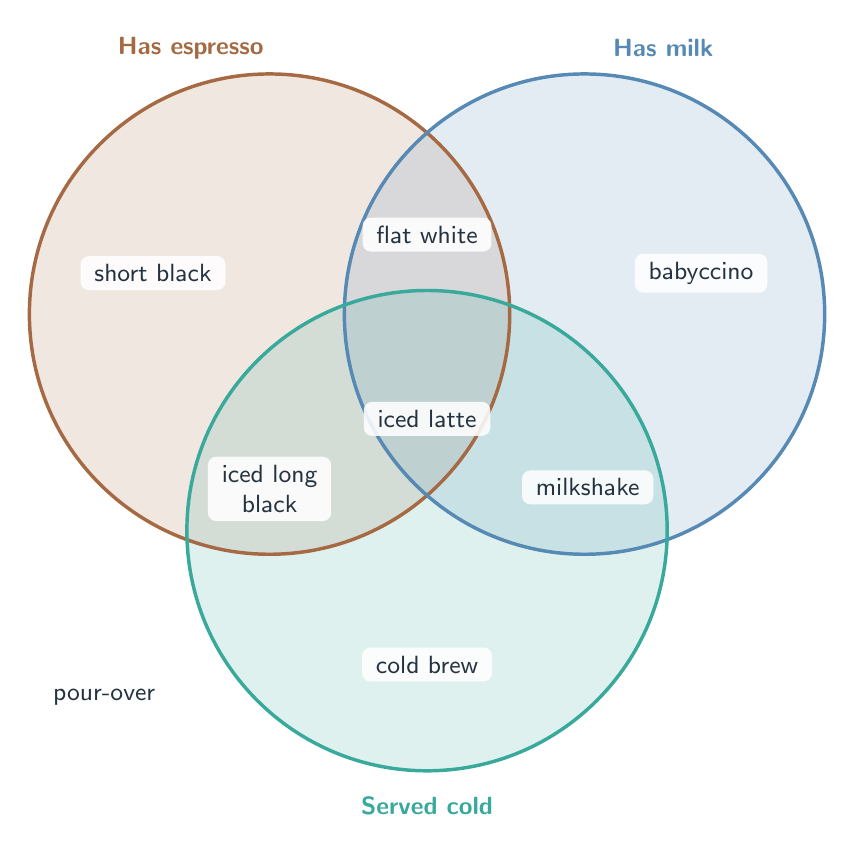
\begin{tikzpicture}[font=\sffamily, text=ink]
  % Three ingredients / serving attributes; transparent fills show overlaps.
  \fill[espresso,opacity=.16] (-2,1.2) circle (3.05);
  \fill[milk,opacity=.16] (2,1.2) circle (3.05);
  \fill[cold,opacity=.16] (0,-1.55) circle (3.05);
  \draw[espresso,line width=1.25pt] (-2,1.2) circle (3.05);
  \draw[milk,line width=1.25pt] (2,1.2) circle (3.05);
  \draw[cold,line width=1.25pt] (0,-1.55) circle (3.05);

  % Circle names sit just beyond the edges, leaving the contents uncluttered.
  \node[font=\sffamily\bfseries\small,espresso] at (-3.0,4.58) {Has espresso};
  \node[font=\sffamily\bfseries\small,milk] at (3.0,4.58) {Has milk};
  \node[font=\sffamily\bfseries\small,cold] at (0,-5.04) {Served cold};

  % One drink in each of the seven interior regions.
  \tikzset{drink/.style={font=\sffamily\small,align=center,fill=white,fill opacity=.87,text opacity=1,rounded corners=3pt,inner xsep=5pt,inner ysep=3pt}}
  \node[drink] at (-3.48,1.72) {short black};
  \node[drink] at (3.48,1.72) {babyccino};
  \node[drink] at (0,-3.25) {cold brew};
  \node[drink] at (0,2.21) {flat white};
  \node[drink] at (-2.0,-1.02) {iced long\\black};
  \node[drink] at (2.04,-1.00) {milkshake};
  \node[drink] at (0,-.13) {iced latte};

  % A pour-over is neither espresso-based, milky, nor served cold.
  \node[drink] at (-4.1,-3.67) {pour-over};
\end{tikzpicture}
\end{document}
